    The proposed algorithm of Abdelsalam et al. \cite{this} is composed of two phases. First is the use of Binary Real Coded Genetic Algorithm (BRCGA) to approximate the near optimal solution to the problem. While the second is the application of local search to the solutions approximated by the BRCGA to improve the solution quality. The reason of using local search as a finishing process for the algorithm is because local search method finds the nearest local optimal solution from the initial solution from the BRCGA. The step by step process of the proposed algorithm is illustrated below.
            
        \section{Encoding}
            \par Encoding marks the start of the BRCGA. Before the genetic algorithm can be put into work, the chromosomes must be encoded to determine how will the fitness of each individual be computed. For the problem in the study of Abdelsalam et al., a chromosome is encoded as shown In Figure \ref{encoding}. From the name itself of the first phase of the proposed algorithm, the chromosome has a binary matrix and a real matrix. The binary matrix is used to mark the positions on the wind farms where wind turbines are present – a value of 1 means a presence of wind turbine on that position while 0 means an absence of wind turbine. The real matrix is used to store the power output of a wind turbine in the wind farm. If a wind turbine is marked present in a location in the binary matrix then the same location in the real matrix will have a value (power output) of greater than zero, otherwise if there is no wind turbine then the power output is zero.
                    
            \begin{figure}[h]
                \centering
                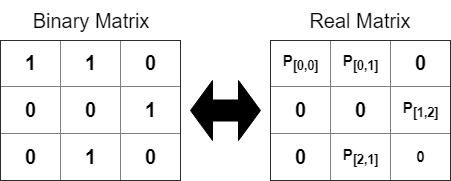
\includegraphics[width=100mm]{Figures/encoding.png}
                \caption{Structure of the chromosome to be used for the algorithm}
                \label{encoding}
            \end{figure}
            
            In Figure \ref{encoding}, since the matrix has 3 rows and 3 columns, the wind farm has a dimension of $600m$ by $600m$. Moreover, it can be seen that there are $N=4$ turbines (marked as "1" in the binary matrix from the figure) located at $(0,0)$, $(0,1)$, $(1,2)$ and $(2,1)$ having power outputs (as shown in the real matrix of Figure \ref{encoding}) of $P_{[0,0]}$, $P_{[0,1]}$, $P_{[1,2]}$ and $P_{[2,1]}$, respectively.
            
        \section{Initialization}
            \par The initialization process is basically creating the first generation of chromosomes, each having random genetic characteristics. Each chromosome having $n\;by\;n$ binary and real matrices will have a total of $n^2$ genes (cells in the matrix) for the binary matrix and another $n^2$ genes for the real matrix where each gene of the binary matrix will have a random value of either "0" or "1". The pseudocode of the initialization of each chromosome is shown below.
                    
                    \singlespacing
        \begin{lstlisting}
            // Initialize the binary matrix with no turbines
            foreach element in binary_matrix
                element = 0
            end foreach
            
            i = 0 // Mark the number of assigned turbines
            while i < N
                // Find a random cell of the matrix
                Let x = a random element in binary_matrix
                if x = 0
                    // If that cell has a value of zero (no turbine), assign value of "1"
                    x = 1
                    i = i + 1 // Increment the number of turbines assigned to the farm
                end if
            end while
        \end{lstlisting}
        \doublespacing
        
        \section{Creation of new generation}
            \par The main goal of a genetic algorithm is to repeatedly create a new generation of chromosomes until the generation where the chromosomes have common genetic characteristics is reached or the maximum number of generations is reached. From a previous generation, the next generation is created through fitness evaluation, selection, crossover, mutation and repairing.
            \begin{enumerate}
                 \item \textbf{Fitness Evaluation}
                    \par Before using the previous generation to create the next generation, the fitness of each chromosome must be evaluated to determine their survival. The goal of the algorithm is to minimize the fitness of each chromosome, where the fitness of the chromosome is the maximum possible power output of the whole wind farm and the minimum possible cost per unit time of the wind turbines, hence can be expressed as
                    \begin{equation}
                        Objective = \frac{Cost_{tot}}{P_{tot}}
                    \end{equation}
                    where $P_{tot}$ is the total power produced by the wind farm or sum of the power produced by each wind turbine for a year, and $Cost_{tot}$ is the cost/year of the whole wind farm. Mosetti et al. \cite{windturbine5} assumed that the non-dimensionalized cost/year of a single wind turbine is 1 and that a maximum cost reduction of 1/3 for every additional wind turbine, hence given $N$ wind turbines installed in the wind farm, the cost/year of each turbine is given by
                    \begin{equation} \label{cost}
                        Cost = \frac{2}{3} + \frac{1}{3}e^{-0.00174N^2}
                    \end{equation}
                    
                    Note that from the formula for the cost of each turbine given by equation \ref{cost}, if the number of turbine is $N=1$ then the cost of that single turbine is $Cost=0.999420504307\approx 1$, and if the number of wind turbines installed increases then the cost of each turbine approaches $\frac{2}{3}$, or
                    \begin{equation}
                        \lim_{N\to\infty} Cost = \lim_{N\to\infty}\Bigg(\frac{2}{3} + \frac{1}{3}e^{-0.00174N^2}\Bigg)=0.6666666667\approx\frac{2}{3}
                    \end{equation}
                    Hence, the assumption of Mosetti et al. \cite{windturbine5} is met. Therefore, the total cost/year of the whole wind farm with $N$ installed wind turbines is
                    \begin{equation}
                        Cost_{tot} = N\Bigg(\frac{2}{3} + \frac{1}{3}e^{-0.00174N^2}\Bigg)
                    \end{equation}
                    
                    Consequently, the power produced by a wind turbine depends on the speed of the wind that passes through that wind turbine and the speed of the wind is always affected by the wake of upstream wind turbines. Therefore, it implies that to maximize the power output is to maximize the wind speed by minimizing the wake effect.
                    
                    The first step of computing the fitness of a chromosome is to determine the wake interaction between the wind turbines in the wind farm. That is for every wind turbine, the goal is to find all other wind turbines which are under its wake. The process on how to determine when a downstream turbine is influenced under wake of an upstream wind turbine is discussed in section \ref{wakeModel}. After the multiple wake interactions had been identified, the next step is to compute the wind speed through each wind turbines using the Sum of Squares Method and modified Jensen's Wake Model and compute the extracted wind power. Note that power produced is different for different types of wind turbines experiencing the same wind speed.
                
                \item \textbf{Tournament Selection}
                    \par Selection is where a number of individuals (chromosomes) are chosen to be parents and to be part of the next generation. Let $m$ be the tournament size and the idea behind tournament selection is that $m$ number of chromosomes are chosen to be the competitors of a tournament and the most fit competitor wins the tournament. Note that a chromosome which already joined previous tournaments can no longer join future tournaments. For a generation of population size $S$ and crossover rate of $rate_{cross}$, it is expected that there will be $\left \lceil{S\cdot(1-rate_{cross})}\right \rceil$ tournaments to produce $\left \lceil{S\cdot(1-rate_{cross})}\right \rceil$ parents. Note that the crossover rate $rate_{cross}$ tells what part of the population is created through crossover. Therefore, if a chromosome can only participate in only one tournament then the tournament size should be
                    \begin{equation}
                        m=\left \lfloor{\frac{S}{\left \lceil{S\cdot(1-rate_{cross})}\right \rceil}}\right \rfloor
                    \end{equation}
                    For example, for a generation of population size $S=10$ and a crossover rate of $rate_{cross}=0.67$, the tournament size would be
                    \begin{equation}
                        m=\left \lfloor{\frac{10}{\left \lceil{10\cdot(1-0.67)}\right \rceil}}\right \rfloor=2
                    \end{equation}
                    
                    The significance of using tournament as a type of chromosome selection method is to preserve the diversity of the whole generation because all of the chromosomes are expected to be part of the tournament thus the algorithm prevents premature convergence. Once the parents are selected, these chromosomes are used to create offspring which will comprise the $[rate_{cross}]\cdot100\;\%$ of the next generation, and these parents becomes part of the next generation, comprising the other $[(1-rate_{cross})\cdot100]\;\%$.
                
                \item \textbf{Uniform Crossover}
                    \begin{figure}[h]
                        \centering
                        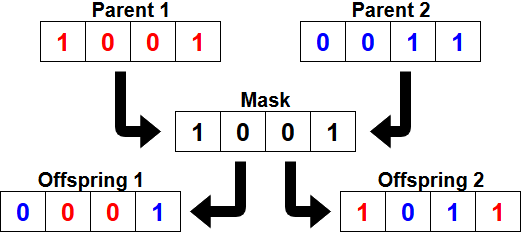
\includegraphics[width=130mm]{Figures/crossover.png}
                        \caption{Crossover of two $1\;by\;4$ parents to produce two new offspring}
                        \label{crossover}
                    \end{figure}
                    \par From the list of chromosomes chosen by tournament selection, a random pair will be removed from the list and used as the parents for crossover. Uniform crossover means the genes of both parents are exchanged uniformly, producing two new offspring. To begin, a random mask is generated. A random mask is a binary matrix, having the same size with the binary matrices of the parents having random elements. The random mask determines whether the parents would exchange bits or not. From the mask, "1" means a parent will exchange genes for the two offspring while "0" means the genes of the offspring will be the same as of the parents as shown in figure \ref{crossover}. Below is the pseudocode of the uniform crossover given a random mask.
                    
        \singlespacing
        \begin{lstlisting}
        Let Pgenes1 = list of genes of first parent
        Let Pgenes2 = list of genes of second parent
        Let Ogenes1 = list of genes of first offspring  // Initially elements are null
        Let Ogenes2 = list of genes of second offspring // Initially elements are null
        Let mask = list of genes of the random mask     // Randomly generated
        
        Let i = 1
        while i is less than or equal size of Pgenes1 or Pgenes2
            if ith element of mask is 1
                ith element of Ogenes1 = ith element of Pgenes2
                ith element of Ogenes2 = ith element of Pgenes1
            else
                ith element of Ogenes1 = ith element of Pgenes1
                ith element of Ogenes2 = ith element of Pgenes2
            end else-if
            i = i+1 // Moves to the next position on the lists
        end while
        \end{lstlisting}
        \doublespacing
                    
                \item \textbf{One Point Mutation}
                    \begin{figure}[h]
                        \centering
                        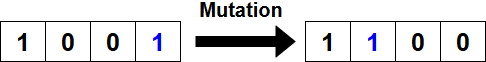
\includegraphics[width=130mm]{Figures/mutation.png}
                        \caption{Sample of One Point Mutation}
                        \label{mutate}
                    \end{figure}
                    \par After the crossover has been done, the next generation is now complete. But before that, the resulting population will proceed for the process called One Point Mutation. Mutation is an important step in the genetic algorithm as it prevents premature convergence. Each individual in the population have equal chances, called the mutation rate $rate_{mutate}$, of being mutated. If a chromosome mutates, a random gene with value 1 from its binary matrix is changed to 0 and a random gene with value 0 from its binary matrix is changed to 1, see Figure \ref{mutate}. This means that when a mutation happens, a wind turbine from the wind farm will be moved to another location in the wind farm assuming that this new position is empty. Below is the pseudocode on how the one point mutation is implemented.
                    
        \singlespacing
        \begin{lstlisting}
        Let mt = mutation rate
        Let x = random value from 0 to 1
        
        if x < mt
            Let i_o = random location in the binary matrix with value 1
            Let i_f = random location in the binary matrix with value 0
            i_o = 0
            i_f = 1
        end if
        \end{lstlisting}
        \doublespacing
                    
                \item \textbf{Repairing}
                    \par There is not always an assurance that the crossover will return a feasible chromosome. A chromosome is said to be feasible if the number of genes with value of 1 in its binary matrix is the same as $N$ or the desired number of wind turbines for the wind farm, otherwise it is infeasible. If a chromosome in the population is infeasible then it must be repaired. To repair a chromosome, if it has too much number of genes with value of 1 in the binary matrix, then repeatedly change a random gene with value of 1 in the binary matrix to a value of 0 until the desired number of turbines $N$ is met; else if it has too less number of genes with value of 1 in the binary matrix, then repeatedly change a random gene with value of 0 in the binary matrix to a value of 1 until the desired number of turbines $N$ is met. Below id the pseudocode of repairing a chromosome.
                   
        \singlespacing 
        \begin{lstlisting}
        Let N = desired number of turbines for the wind farm
        Let x = number of genes with value 0 in the binary matrix
        while N is not equal to x
            if x < N
                Let i = random gene with value 0 in the binary matrix
                i = 1
                x = x + 1
            else
                Let i = random gene with value 1 in the binary matrix
                i = 0
                x = x - 1
            end if
         end while
        \end{lstlisting}
        \doublespacing
                    
                    This shows that if the wind farm, which is represented by the infeasible chromosome, has too much wind turbines then a random wind turbine is removed, else if it has too less wind turbine, a wind turbine is added in random locations.
            \end{enumerate}
            
        \section{Local Search}
            \par Local search algorithm is one of the fundamental heuristic methods for solving computational problems. It starts with a finite set of candidate solutions $s$ which is a subset of all the possible solutions or the search space $S$. Then, it iteratively finds the neighboring solution for each candidate solution to gradually improve $s$ \cite{localsearch1}. A \textbf{neighboring solution} $k$ to an initial solution $k_o$ is a position in $S$ that is one step away from $k_o$. The search will come to a stop when there is no longer a superior neighboring solution $y$. It is called a \textbf{superior neighboring solution} if it better satisfies the problem than the initial solution \cite{localsearch2}.
            
            \begin{figure}[h]
                \centering
                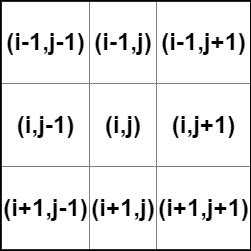
\includegraphics[width=55mm]{Figures/adjacentLoc.png}
                \caption{Adjacent locations to $(i,j)$}
                \label{adjacentLoc}
            \end{figure}
            
            After the first phase (BRCGA) of the proposed algorithm is finished, local search is applied to enhance the set of solutions provided by the BRCGA. A neighboring solution from an initial solution is a solution where a wind turbine is moved to a location adjacent to the initial location. This means that from the binary matrix, a gene with value of 1 on location $(i,j)$ can be moved to locations $(i-1,j-1)$, $(i-1,j)$, $(i-1,j+1)$, $(i,j-1)$, $(i,j+1)$, $(i+1,j-1)$, $(i+1,j)$ and $(i+1,j+1)$ as shown in Figure \ref{adjacentLoc}, assuming that these locations exist and are not empty.